\section{Blockchain} \label{sec:Blockchain}

\subsection{Structure} \label{sec:BlockchainStructure}
The blockchain is a record of all transactions that have occured in the Bitcoin system and is shared by every node in it. Its main purpose is to infer spending for all transaction outputs. The novelty of Bitcoin lies, among other things, in how the blockchain is structured in order to guarantee chronological ordering of transactions and prevent double-spending in a distributed network.

As described in Sect. \ref{sec:Blocks}, every block in the blockchain refers to the hash of a previous block. This imposes a chronological order on blocks and therefore transactions as well, since it is not possible to create a valid hash of the previous block header prior to its existence.

Furthermore, each block includes the solution to a proof-of-work puzzle of a certain difficulty. The computational power involved in solving the proof-of-work puzzle for each block is used as a voting scheme to enable all nodes in the network to collectively agree on a version of the blockchain. Nodes collectively agree on the blockchain that involved the highest accumulated computational effort to be created. Thus, modifying a block in the chain would require an adversary to recompute proof-of-work puzzles of equal or greater computational effort than the ones from that block up until the newest block. In order to achieve that, the adversary would have to computationally outperform the majority of the network, which is considered infeasible.
\begin{figure}[ht!]
 \centering
 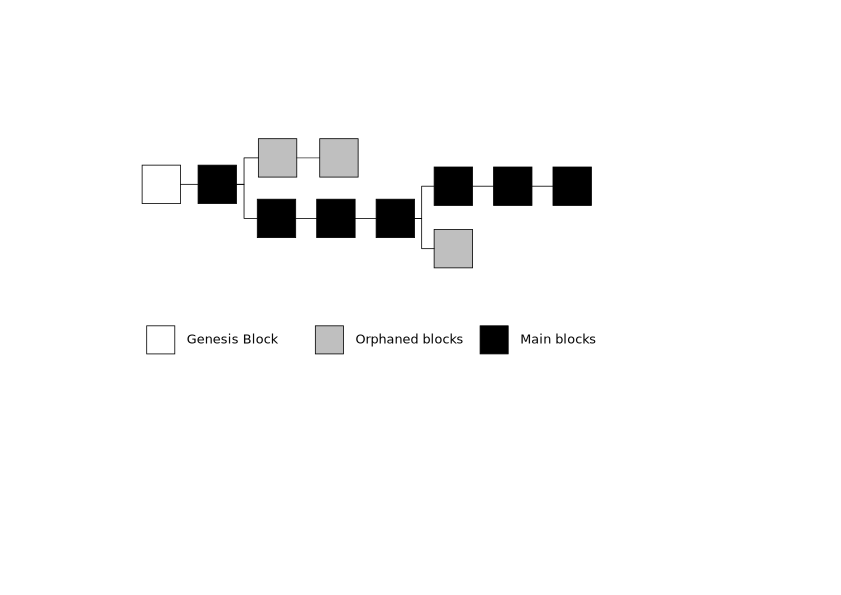
\includegraphics[scale=0.6]{images/Blockchain.pdf}
 \caption{Blockchain}
 \label{figure:Blockchain}
\end{figure}

\noindent
Clearly, since nodes in the network compete in a randomized process to successfully solve the proof-of-work puzzle and gain a reward, there is a chance that two different blocks are mined simultaneously and the chain forks. In this case nodes will accept whichever block they have received first and continue building the chain upon that block. If another block is found, then the branch that was used will become the main blockchain. If this happens, all valid transactions within the shorter chain are re-added to the pool of queued transactions. The resulting structure resembles what is depicted in Fig. \ref{figure:Blockchain}, the white block being the first block ever mined, also referred to as the genesis block, the black chain representing the main chain and grey blocks being orphans due to forking.

\subsection{Mining} \label{sec:Mining}

\subsubsection*{Procedure}
The process of finding a valid block is called \emph{mining} whereas nodes that participate in that process are called \emph{miners}. As described in \cite{Clark_BitcoinInternals}, mining nodes perform the following steps in an endless loop:

\begin{enumerate}[label=\arabic*), leftmargin=1cm]
\item Collect all broadcasted transactions and validate whether they satisfy the miner's self-defined policy. Typically, a transaction includes a transaction fee that functions as an incentive for the miner to include it in the block. However, if it does not, then it is up to the miner to decide what to do with it.
\item Verify all transactions that are to be included in the block. Transactions are verified as described in Sect. \ref{sec:Script} and it is checked whether their inputs have been previously spent.
\item Select the most recent block on the longest path in the blockchain, i.e. the path that involves most accumulated computational effort, and insert the hash of the block header into the new block.
\item Solve the proof-of-work problem as described below and broadcast the solution. Should another node solve the proof-of-work problem before, then the block is first validated - the proof-of-work solution is checked and all transactions included in the block are verified. If it passes these controls then the cycle is repeated. Note that if there are transactions that have not been included in the new block then they are saved and included in the next cycle.
\end{enumerate}


\subsubsection*{Proof-of-Work}
During mining a miner attempts to find a block header whose double-SHA256 hash lies below the target value $T$. In order to succeed he needs a certain degree of freedom in the block header that allows him to compute various hashes without interfering with its semantics. Hence, two fields are used as a source of randomness - the nonce field (\textit{nNonce}) in the block header itself and the coinbase field (\textit{coinbase}) in the coinbase transaction, which indirectly changes the Merkle root (\textit{HashMerkleRoot}) in the block header. The process of finding a proof-of-work can then be divided into three steps:

\begin{enumerate}[label=\arabic*), leftmargin=1cm]
\item Set the nonce field and the coinbase field to values of one's choosing.
\item Compute the hash of the block header as
\begin{equation}
SHA256^{2}(nVersion||HashPrevBlock||HashMerkleRoot||nTime||nBits||nNonce)
\label{eqn:HashBlock}
\end{equation}
\item Reverse the byte order of the computed hash and check whether its value $\mathit{H}$ lies below the current target value $\mathit{T}$ (stored in compact format in the \textit{nBits} field):
\begin{equation}
H \leq T
\end{equation}

\end{enumerate}

\noindent
This process is repeated for various values of \textit{nNonce} and \textit{coinbase} until a valid solution is found. Typically, for efficiency reasons, all possible values of the nonce field are evaluated before changes to the coinbase field are made.